\documentclass{article}
\usepackage{graphicx}
\usepackage{subcaption}

\begin{document}

\section{Attempt 2}

\begin{figure}[ht]

    \centering
    \begin{subfigure}{0.33\textwidth}
      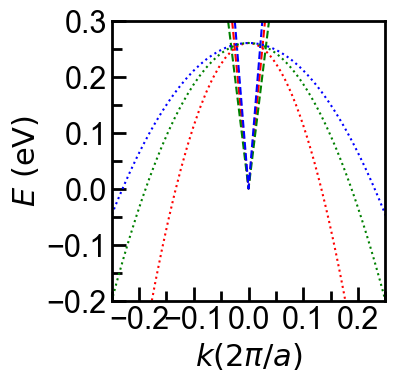
\includegraphics[width=\textwidth]{../Fig2BM-typeI.png}
      \caption{}
    \end{subfigure}
    \hfil
    \begin{subfigure}{0.33\textwidth}
      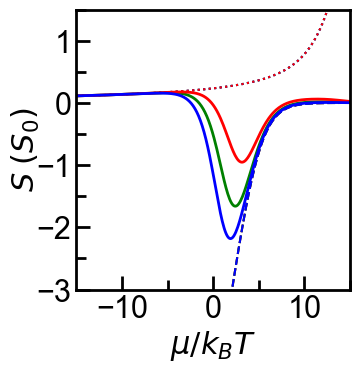
\includegraphics[width=\textwidth]{../Seebeck.png}
      \caption{}
    \end{subfigure}
    \hfil
    \begin{subfigure}{0.33\textwidth}
      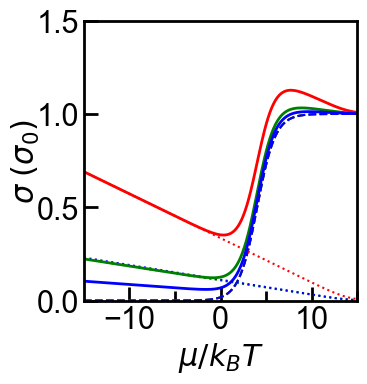
\includegraphics[width=\textwidth]{../conductivity.png}
      \caption{}
    \end{subfigure}
    \begin{subfigure}{0.33\textwidth}
      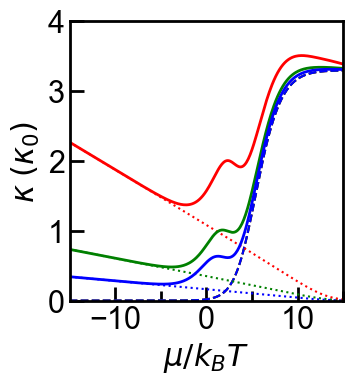
\includegraphics[width=\textwidth]{../Thermal.png}
      \caption{}
    \end{subfigure}
    \hfil
    \begin{subfigure}{0.33\textwidth}
      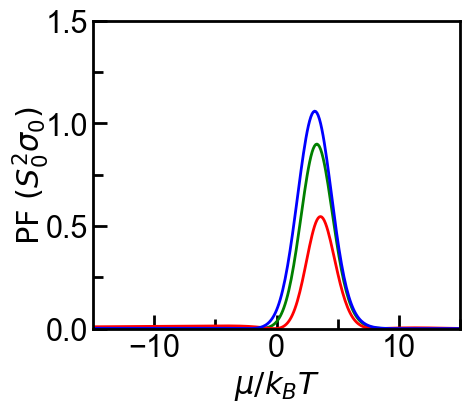
\includegraphics[width=\textwidth]{../PF.png}
      \caption{}
    \end{subfigure}
    \hfil
    \begin{subfigure}{0.33\textwidth}
      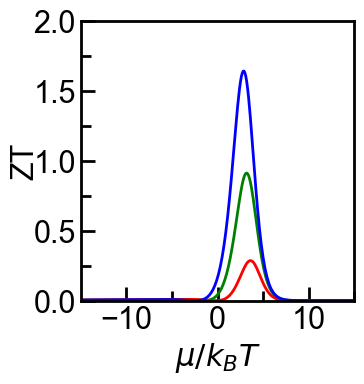
\includegraphics[width=\textwidth]{../ZT.png}
      \caption{}
    \end{subfigure}

\caption{Thermoelectric properties of TiS.(a) TiS Model Band Structure (b) Seebeck, (c) Conductivity, (d) Thermal, (e)PF, and (f) ZT}
\label{fig:six_images_with_horizontal_space}
\end{figure}

\end{document}